% no notes
\documentclass{beamer}
% notes and slides
%\documentclass[notes]{beamer}
% notes only
%\documentclass[notes=only]{beamer}
\usepackage{graphicx} % Allows including images
\usepackage{booktabs} % Allows the use of \toprule, \midrule and \bottomrule in tables
\usepackage{multirow}
\usepackage{multimedia}
\usepackage{tikz}
\usepackage{circuitikz}
\usepackage{url}
\usepackage{pgfplots}
\pgfplotsset{compat=newest}
\usepgfplotslibrary{groupplots,dateplot}
\usetikzlibrary{patterns,shapes.arrows}
\usepackage{standalone}
\usepackage{adjustbox}
\usepackage{lmodern}
\usepackage{pgfplots}
\usepackage{amsmath}
\usepackage{amsthm}
\usepackage{multimedia}
\usepackage{standalone}
\usepackage{csquotes}
%\usepackage{hyperlink}
%\usepackage{url}

% python listings
% from https://tex.stackexchange.com/questions/83882/how-to-highlight-python-syntax-in-latex-listings-lstinputlistings-command
% Default fixed font does not support bold face
\DeclareFixedFont{\ttb}{T1}{txtt}{bx}{n}{12} % for bold
\DeclareFixedFont{\ttm}{T1}{txtt}{m}{n}{12}  % for normal

% Custom colors
\usepackage{color}
\definecolor{deepblue}{rgb}{0,0,0.5}
\definecolor{deepred}{rgb}{0.6,0,0}
\definecolor{deepgreen}{rgb}{0,0.5,0}

\usepackage{listings}

% Python style for highlighting
\newcommand\pythonstyle{\lstset{
language=Python,
basicstyle=\ttm,
morekeywords={self},              % Add keywords here
keywordstyle=\ttb\color{deepblue},
emph={MyClass,__init__},          % Custom highlighting
emphstyle=\ttb\color{deepred},    % Custom highlighting style
stringstyle=\color{deepgreen},
frame=tb,                         % Any extra options here
showstringspaces=false
}}


% Python environment
\lstnewenvironment{python}[1][]
{
\pythonstyle
\lstset{#1}
}
{}

% Python for external files
\newcommand\pythonexternal[2][]{{
\pythonstyle
\lstinputlisting[#1]{#2}}}

% Python for inline
\newcommand\pythoninline[1]{{\pythonstyle\lstinline!#1!}}

\PassOptionsToPackage{american}{babel} % change this to your language(s), main language last
% Spanish languages need extra options in order to work with this template
% \PassOptionsToPackage{spanish,es-lcroman}{babel}
\usepackage{babel}

\PassOptionsToPackage{%
  backend=biber,bibencoding=utf8, %instead of bibtex
  %backend=bibtex8,bibencoding=ascii,%
  language=auto,%
  style=numeric-comp,%
  %style=authoryear-comp, % Author 1999, 2010
  %bibstyle=authoryear,dashed=false, % dashed: substitute rep. author with ---
  style=alphabetic,
  sorting=nyt, % name, year, title
  maxbibnames=10, % default: 3, et al.
  %backref=true,%
  %natbib=true % natbib compatibility mode (\citep and \citet still work)
}{biblatex}
\usepackage{biblatex}

\addbibresource{bib.bib}

\usetheme{metropolis}           % Use metropolis theme
\setbeamertemplate{caption}[default]
\title{Introduction to Neural Networks}
\date{\today}
\institute{High-Performance Computing and Analytics Lab}
\author{Moritz Wolter}

\titlegraphic{
\includegraphics[width=2.00cm]{UNI_Bonn_Logo_Standard_RZ.pdf}}

\begin{document}
    \maketitle

    \begin{frame}
    \frametitle{Overview} 
    \tableofcontents
    \end{frame}

    \section{Neural networks}
    \begin{frame}{The wonders of the human visual system}
      \begin{figure}
        \includestandalone[width=0.9\linewidth,height=1.5cm]{./figures/mnist_sequence}
        \caption{Most humans effortlessly recognize the digits \texttt{5 0 4 1 9 2 1 3}.}
      \end{figure}
    \end{frame}

    \begin{frame}{Biological motivation}
      \centering
      \begin{figure}
        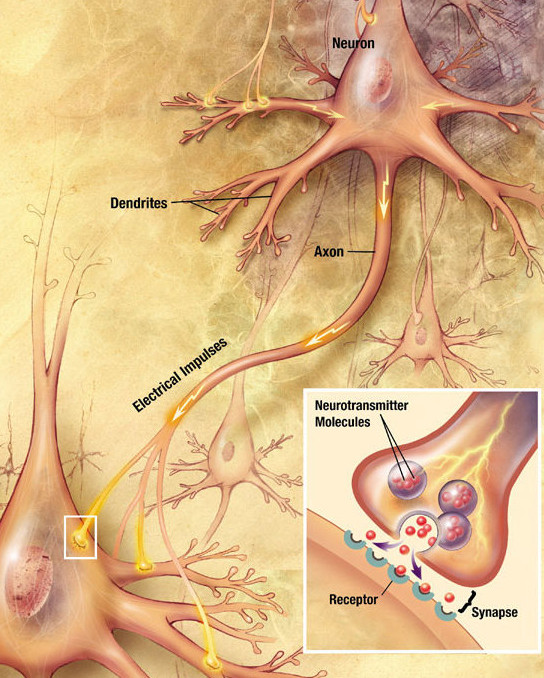
\includegraphics[scale=0.3]{./figures/Chemical_synapse_schema_cropped}  
      \end{figure}
      Image source: en.wikipedia.org
      %Image source: \url{https://en.wikipedia.org/wiki/Neuron#/media/File:Chemical_synapse_schema_cropped.jpg} 
    \note{
      \begin{itemize}
        \item A Human brain contains approximately 86 billion neurons.
        \item $10^{14}$ to $10^{15}$ synapses connect these neurons.
        \item Neurons receive inputs from dendrites.
        \item and can produce output signals along its axon.
        \item Axons connect neurons, modeled by weighting inputs $wx$.
        \item Neuron inputs can be inhibitive (negative weight) or
        \item excitatory (positive weight).
        \item If enough inputs excite a neuron, it fires.
        \item The activation function aims to mimic this behavior.
        \item Even though neural networks started out as biologically motivated,
        \item engineering efforts have since diverged from biology.
      \end{itemize}
    }
    \end{frame}


    \begin{frame}{The perceptron}
      Can computers recognize digits? Mimic biological neurons,
      \begin{figure}
        \includestandalone[scale=.575]{./figures/perceptron}
      \end{figure}
      Formally a single perceptron is defined as
      \begin{align}
        f(\mathbf{w}^T \mathbf{x} + b) = h
      \end{align}
      with $\mathbf{w} \in \mathbb{R}^n$, $\mathbf{x} \in \mathbb{R}^n$ and $h,b \in \mathbb{R}$. 
    \end{frame}

    \begin{frame}{The activation function $f$}
      Two popular choices for the activation function $f$.
      \begin{figure}
        \includestandalone[width=0.49\linewidth]{./figures/sigmoid}
        \includestandalone[width=0.49\linewidth]{./figures/ReLU}
      \end{figure}
    \end{frame}

    \begin{frame}{Arrays of perceptrons}
      Let's extend the definition to cover an array of perceptrons:
      \begin{figure}
        \includestandalone[scale=0.5]{./figures/perceptron_array}
      \end{figure}
      Every input is connected to every neuron. In matrix language, this turns into
      \begin{align}
        \bar{\mathbf{h}} &= \mathbf{W}\mathbf{x} + \mathbf{b}, & \mathbf{h} = f(\bar{\mathbf{h}}).
      \end{align}
      With $\mathbf{W} \in \mathbb{R}^{m,n}$, $\mathbf{x} \in \mathbb{R}^{n}$, $\mathbf{b} \in \mathbb{R}^{m}$, and $\mathbf{h}, \bar{\mathbf{h}} \in \mathbb{R}^m$.
    \end{frame}

    \begin{frame}{The loss function}
      To choose weights for the network, we require a quality measure. \\
      We already saw the squared error cost function,
      \begin{align}
        C_{\text{se}} = \frac{1}{2} \sum_{k=1}^{n} (\mathbf{h}_k - \mathbf{y}_k)^2 = \frac{1}{2} (\mathbf{h} - \mathbf{y})^T(\mathbf{h} - \mathbf{y})
      \end{align}
      This function measures the squared distance from each desired output.
      $\mathbf{y}$ denotes the desired labels, and $\mathbf{h}$ represents network output.
    \end{frame}


    \begin{frame}{The gradient of the se-cost-function}
      Both the squared error loss function and our dense layer are differentiable. 
      \begin{align}
        \frac{\partial C_{\text{se}}}{\partial \mathbf{h}} = \mathbf{h} - \mathbf{y} = \triangle_{\text{se}}
      \end{align}
      The $\triangle$ symbol will re-appear. It always indicates incoming gradient information from above.
      If the labels are a vector of shape $\mathbb{R}^m$, $\triangle$ and the network output $\mathbf{h}$ must share 
      this dimension.
    \end{frame}

    \begin{frame}{The gradient of a dense layer}
      The chain rule tells us the gradients for the dense layer~\cite{nielsen2015neural}
      \begin{align}
        \delta \mathbf{W} &= [f'(\bar{\mathbf{h}}) \odot \triangle]\mathbf{x}^T, &  \delta \mathbf{b} = f'(\bar{\mathbf{h}}) \odot \triangle, \\
        \delta \mathbf{x} &= \mathbf{W}^T [f'(\bar{\mathbf{h}}) \odot \triangle],
      \end{align}
      where $\odot$ is the element-wise product. $\delta$ denotes the cost function gradient for the value following it \cite{greff2016lstm}. \\
      With $\delta \mathbf{W} \in \mathbb{R}^{m,n}$, $\delta \mathbf{x} \in \mathbb{R}^{n}$ and $\delta \mathbf{b} \in \mathbb{R}^{m}$.
      \textbf{Modern libraries will take care of these computations for you!} \\
      
      \note<1>{
        On the board, derive:
        Recall the chain rule $(g(h(x)))' = g'(h(x)) \cdot h'(x)$.
        For the activation function, we have,
        \begin{align}
          \mathbf{h} &= f(\bar{\mathbf{h}}) \\
          \Rightarrow \delta \bar{\mathbf{h}} &= f'(\bar{\mathbf{h}}) \odot \triangle
        \end{align}
        For the weight matrix,
        \begin{align}
          \bar{\mathbf{h}} &= \mathbf{W}\mathbf{x} + \mathbf{b} \\
          \Rightarrow \delta \mathbf{W} &= \delta \bar{\mathbf{h}} \mathbf{x}^T = [f'(\bar{\mathbf{h}}) \odot \triangle] \mathbf{x}^T
        \end{align}
        For the bias,
        \begin{align}
          \bar{\mathbf{h}}  &= \mathbf{W}\mathbf{x} + \mathbf{b} \\
          \Rightarrow \delta \mathbf{b} &= 1 \odot \delta \bar{\mathbf{h}} = [f'(\bar{\mathbf{h}}) \odot \triangle]
        \end{align}
      }
    \end{frame}

    \begin{frame}{Derivatives of our activation functions}
      \begin{align}
        \sigma'(x) = \sigma(x) \cdot (1 - \sigma(x)) \\
        \text{ReLU}'(x) = H(x) 
      \end{align}
      \begin{figure}
        \includestandalone[width=0.49\linewidth]{./figures/sigmoid_prime}
        \includestandalone[width=0.447\linewidth]{./figures/relu_prime}
      \end{figure}
    \end{frame}

    \begin{frame}{Perceptrons for functions}
      The network components described this far already allow function learning.
      Given a noisy input signal $x \in \mathbb{R}^{m}$ and a ground through output $\mathbf{y} \in \mathbb{R}^m$,
      define,
      \begin{align}
        \mathbf{h}_1 = \sigma(\mathbf{W}\mathbf{x} + \mathbf{b}) \\
        \mathbf{o} = \mathbf{W}_{\text{proj}}\mathbf{h}_1
      \end{align}
      With $\mathbf{W} \in \mathbb{R}^{m,n}$, $\mathbf{x} \in \mathbb{R}^{n}$ and $\mathbf{b} \in \mathbb{R}^{m}$.
      $m$ and $n$ denote the number of neurons and the input signal length.
      For signal denoising, input and output have the same length.
      Therefore $\mathbf{W}_{\text{proj}} \in \mathbb{R}^{n,m}$.
      $\mathbf{o} \in \mathbb{R}^{n}$ denotes the network output.
    \end{frame}

    \begin{frame}{Denoising a cosine}
      Training works by iteratively descending along the gradients. For $\mathbf{W}$ the weights at the
      next time step $\tau$ are given by,
      \begin{align}
        \mathbf{W}_{\tau + 1} = \mathbf{W}_\tau - \epsilon \cdot \delta\mathbf{W}_{\tau}.
      \end{align}
      The step size is given by $\epsilon \in \mathbb{R}$. At $\tau = 0$, matrix entries are random.
      $\mathcal{U}[-0.1, 0.1]$ is a reasonable choice here.
      The process is the same for all other network components.
    \end{frame}

    \begin{frame}{Denoising a cosine}
      Optimization for 500 steps with 10 neurons, leads to the output below:
      \begin{figure}
        \includestandalone[width=.5\linewidth]{./figures/denoising}
        \caption{The cosine function is shown in blue, a noisy network input in orange, and a denoised network output in green.}
        \end{figure}
    \end{frame}

    \begin{frame}{Summary}
      \begin{itemize}
        \item Artificial neural networks are biologically motivated.
        \item Gradients make it possible to optimize arrays of neurons.
        \item A single array of layers of neurons can solve tasks like denoising a sine.
      \end{itemize}
    \end{frame}


    \section{Classification with neural networks}

    \begin{frame}{Deep multi-layer networks}
      Stack dense layers and activations to create deep networks. \\
      \begin{figure}
        \includestandalone[width=\linewidth]{./figures/multilayer} 
      \end{figure}
    \end{frame}

    \begin{frame}{Backpropagation}
      \begin{figure}
        \includestandalone[width=\linewidth]{./figures/backprop} 
      \end{figure}
    \end{frame}

    \begin{frame}{The cross-entropy loss}
      The cross-entropy loss function is defined as \cite{nielsen2015neural, bishop2006pattern}
      \begin{align} \label{eq:ce}
       C_{\text{ce}}(\mathbf{y}, \mathbf{o}) = -\sum_k^{n_o} [( \mathbf{y}_k  \ln \mathbf{o}_k) 
                                  + (\mathbf{1} - \mathbf{y}_k)
                                     \ln(\mathbf{1} - \mathbf{o}_k)].
      \end{align}
      With $n_o$ the number of output neurons. $\mathbf{y} \in \mathbb{R}^{n_o}$ the desired output and
      $\mathbf{o} \in \mathbb{R}^{n_o}$ the network output.
    \end{frame}

    \begin{frame}{Understanding how cross-entropy works}
      To understand cross entropy let's consider the boundary cases $y=0$ and $y=1$.
      \begin{figure}
        \includestandalone[width=0.49\linewidth]{./figures/ce_label_0}
        \includestandalone[width=0.49\linewidth]{./figures/ce_label_1}
      \end{figure}
    \end{frame}

    \begin{frame}{Gradients and cross-entropy}
      If a sigmoidal activation function produced $\mathbf{o}$ the gradients can be computed using ~\cite{nielsen2015neural,bishop2006pattern}
      \begin{align} 
         \frac{\partial C_{ce}}{\partial \mathbf{h}} 
         = \sigma(\mathbf{o}) - \mathbf{y} = \triangle_{\text{ce}}
      \end{align}
      \note{
        Following \cite{nielsen2015neural}, substitute $\sigma(\mathbf{o})$ into eq~\ref{eq:ce}.
      }
    \end{frame}

    \begin{frame}{The MNIST-Dataset}
      \begin{figure}
        \includestandalone[width=0.9\linewidth,height=1.5cm]{./figures/mnist_sequence}
        \caption{The MNIST-dataset contains 70k images of handwritten digits.}
      \end{figure}
    \end{frame}

    \begin{frame}{Validation and Test data splits}
      \begin{itemize}
        \item To ensure the correct operation of the systems we devise, it is paramount to 
        hold back part of the data for validation and testing.
        \item Before starting to train, split off validation and test data.
        \item The 70k MNIST samples could, for example, be partitioned into 59k training images.
        1k validation images and 10k test images. 
      \end{itemize}
    \end{frame}

    \begin{frame}{Input-preprocessing}
      Standard initializations and learning algorithms assume an approximately standard normal distribution
      of the network inputs. Consequently, we must rescale the data using,
      \begin{align}
        {x}_{ij} = \frac{x_{ij} - \mu}{\sigma}
      \end{align}
      With $\mu$ and $\sigma$ the training set mean and standard deviation.
      For all pixels, $i,j$ up the height and width of every image.
      $b$ denotes the number of data points, and $n$ is the data dimension.
    \end{frame}

    \begin{frame}{The effect of normalization}
      \begin{figure}
      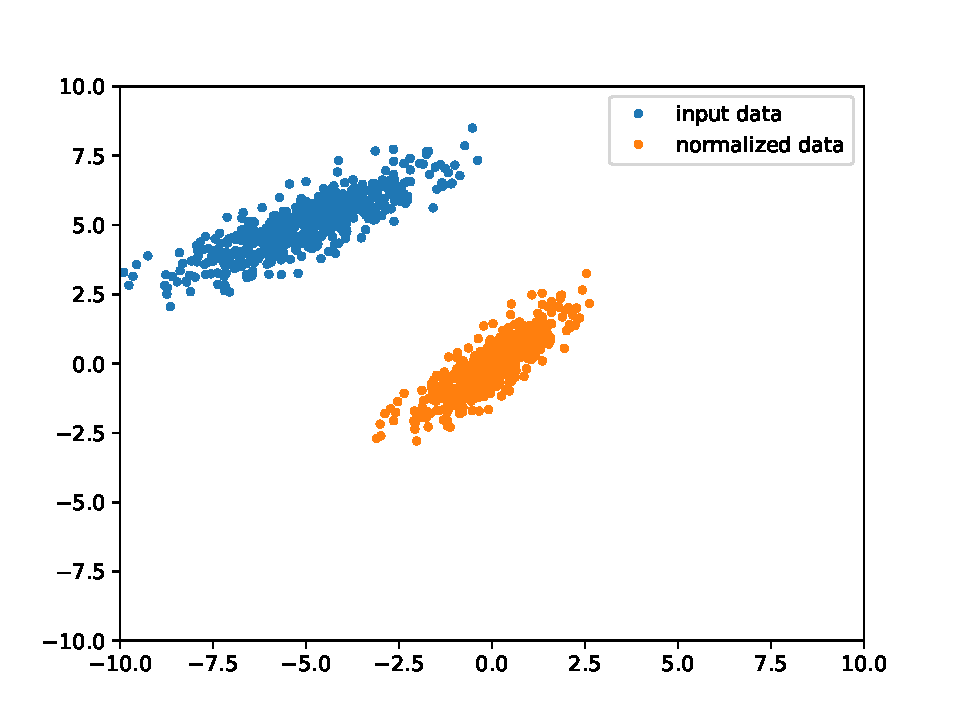
\includegraphics[width=\linewidth]{./figures/normalized.pdf}
      \end{figure}
    \end{frame}

    \begin{frame}{Whitening the inputs \cite{CS231n}}
      Instead of dividing by the standard deviation, rescale the centered data with the singular values of the covariance matrix.
      \begin{align}
        \mathbf{C} = \frac{1}{n} (\mathbf{x} - \mu)^T(\mathbf{x} - \mu)
      \end{align}
      With $n$ as the total number of data points. Next we find $\mathbf{U}\mathbf{\Sigma}\mathbf{V} = \mathbf{C}$.
      After projecting the data via $\mathbf{p} = \mathbf{x}\mathbf{U}$. Whitening now uses the singular values of $\mathbf{C}$ to rescale the data,
      \begin{align}
        p_{ij} = \frac{p_{ij}}{\sqrt{\sigma_j} + \epsilon}
      \end{align}
      With $\epsilon$ i.e. equal to $1e^{-8}$ for numerical stability.
      The operation is repeated for all pixel locations $i,j$ in the input image.
    \end{frame}

    \begin{frame}{The effect of Whitening}
    \begin{figure}
    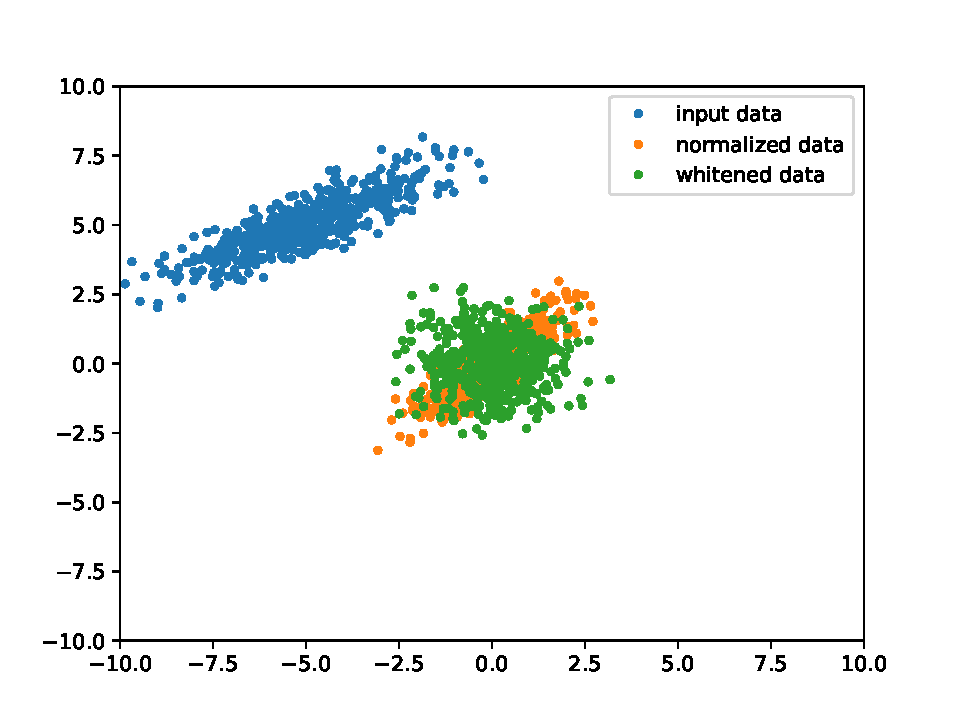
\includegraphics[width=\linewidth]{./figures/whitened.pdf}
      \end{figure}
      Whitening is expensive and sometimes unstable. Consequently, most projects rely on normalization.
    \end{frame}


    \begin{frame}{Label-encoding}
      It has proven useful to have individual output neurons produce probabilities for each class.
      Given integer labels $1,2,3,4, \dots \in \mathbb{Z}$. One-hot encoded label vectors have a one 
      at the label's position and zeros elsewhere. I.e.
      \begin{align}
        \begin{pmatrix}
          1 \\ 0 \\ 0 \\ 0 \\ \vdots
        \end{pmatrix},
        \begin{pmatrix}
          0 \\ 1 \\ 0 \\ 0 \\\vdots
        \end{pmatrix},
        \begin{pmatrix}
          0 \\ 0 \\ 1 \\ 0 \\\vdots
        \end{pmatrix},
        \begin{pmatrix}
          0 \\ 0 \\ 0 \\ 1 \\\vdots
        \end{pmatrix},
        \dots
      \end{align}
      for the integer label sequence above.
    \end{frame}


    \begin{frame}{Batching the data}
      Working with individual data points is not efficient in practice.
      Instead, we would like to process multiple (i.e. 64) samples in parallel. 
      Add a leading batch dimension and rely on broadcasting.

      An additional mean converts the cost of a batch into a scalar.
      In the cross-entropy case:
      \begin{align}
        C_{\text{ce}}(\mathbf{y},\mathbf{o})=-\frac{1}{n_b}\sum_{i=1}^{n_b}\sum_{k=1}^{n_o}[(\mathbf{y}_{i,k}\ln\mathbf{o}_{i,k})+(\mathbf{1}-\mathbf{y}_{i,k})\ln(\mathbf{1}-\mathbf{o}_{i,k})]
      \end{align}
      With $n_o$ the number of output neurons and $n_b$ the batch size.
    \end{frame}

    \begin{frame}{MNIST-Classification}
      Training a three-layer dense network on mnist for five runs leads to:
      \begin{figure}
        \includestandalone[width=0.7\linewidth]{./figures/mnist_runs_plot}
      \end{figure}
    \end{frame}

    \begin{frame}{Conclusion}
      \begin{itemize}
        \item Preprocessing followed by forward passes, backward passes, and testing from the classic training pipeline.
        \item Using the pipeline, artificial neural networks enable computers to make sense of images.
        \item The optimization result depends on the initialization.
        \item The initialization depends on the seed of the pseudorandom number generator.
        \item \textit{Seed-values must be recorded}, to allow reproduction.
        \item Share the results of multiple re-initialized runs, if possible.
      \end{itemize}
    \end{frame}

    \begin{frame}[allowframebreaks]{Literature}
      \printbibliography
    \end{frame}

    \section{Network coding}
    \begin{frame}[fragile]{Networks in Flax}
      Code examples for added implementation fun!! A minimal net:
      \begin{python}
      import jax.numpy as jnp
      from flax import linen as nn

      class Net(nn.Module):
      @nn.compact
      def __call__(self, x):
          x = jnp.reshape(x,
              [x.shape[0], -1])
          x = nn.Dense(10)(x)
          x = nn.sigmoid(x)
          return x
      \end{python}
      Add more layers in our own experiments!!
    \end{frame}

    \begin{frame}[fragile]{Network initialization}
      Initialization requires a key for the pseudorandom number generator.
      \begin{python}
      key = jax.random.PRNGKey(key)
      net = Net()
      variables = net.init(
          key, jnp.ones([batch_size]
          + list(img_data_train.shape[1:])
          + [1])
      )
      \end{python} 
    \end{frame}

    \begin{frame}[fragile]{A forward pass}
      A forward pass through the net requires the weights and an input array.
      \begin{python}
      output = net.apply(
        variables,
        jnp.expand_dims(img_batch, -1)
      )
      \end{python}
    \end{frame}

    \begin{frame}[fragile]{Gradient steps on weight trees} 
      \begin{python}
      weights = jax.tree_util.tree_map(
          update_fun,
          weights, grads
      )
      \end{python} 
      It's useful to use a lambda function here.
      The function should have two arguments \texttt{weights} and \texttt{grads} and return
      \texttt{weights} - \texttt{learning\_rate * grads}. \\
      More information on lambda functions: \\
      \url{https://docs.python.org/3/tutorial/controlflow.html#lambda-expressions} . \\
      More information on the tree maps: \\
      \url{https://jax.readthedocs.io/en/latest/_autosummary/jax.tree_util.tree_map.html}
    \end{frame}

\end{document}
